\documentclass[a4paper,final]{article}
\usepackage{subfig}
\usepackage[dutch]{babel}
\usepackage{minutes}
\usepackage{graphicx}
\usepackage{float}

\title{Notulen 015 overleg team 33}
\author{Guus}
\minutesstyle{header=table, vote=list, contents=true, columns={1}}

\begin{document}
%\selectlanguage{dutch}

\begin{Minutes}{Overleg 014 team 33}
\participant{Freek Verbeek, Bernard van Gastel, Guus Bonnema}
\subtitle{Kennismaking en project toelichting}
\minutetaker{Guus}
\minutesdate{27 november 2014}
\location{Toernooiveld 200, Nijmegen (Mercator gebouw)}

\maketitle% This is where LaTeX makes the title

\newcommand{\w}[1]{\textsc{#1}}

\topic{Introduction}

Dit is een incidenteel overleg ter kennismaking en als secondaire doel een
completer beeld van het project en de projectbelangen te krijgen.

\paragraph{Bernard van Gastel} Bernard is promovendus op basis van derden geldstroom. 
Hij had na zijn studie een eigen bedrijf maar kon de trek naar onderzoek niet weerstaan
en is zijn promotie bij de RU begonnen onder funding van Intel. Hij is nu 3 jaar 
met promotie bezig en heeft 1 jaar te gaan.

\paragraph{Freek Verbeek} Freek is universitair docent aan de RU. 
Hij promoveerde aan het RU in communication fabrics (NoC) en concentreert zich
momenteel op verification tools naast onderwijs en andere onderzoeken.

\paragraph{Guus Bonnema} Guus is OU student met een verleden in IT 
als programmeur in vele job typen waaronder ontwikkelaar en beheerder.

\paragraph{Rolverdeling} Zowel Bernard als Freek zijn actief bij het project
betrokken, maar conform onderlinge afspraak bemoeit Bernard zich naar ons toe
met de inhoud van het project en Freek met de begeleiding. 
Achter de schermen sluiten Freek en Bernard de inhoudelijke aspecten met elkaar kort.
De begeleiding is alleen zaak voor Freek.

Praktisch gezien is Freek meer gericht op de verificatie modules terwijl
Bernard gericht is op het hele project ten behoeve van zijn promotie. Bernard
doet daarnaast actief verificatie modules ontwikkelen en de verification pipeline
faciliteren (zie topic architectuur).

\topic{Onderzoekscontext} Freek licht de doelen van het project toe. Enerzijds
zijn er onderzoekers aan de RU (Radboud Universiteit) die analyse en
verificatie tools maken en daar publicaties over doen.  Anderzijds willen de
onderzoekers hun publicaties aan de man brengen (``Valorisatie'') bij
onderzoekers bij andere universiteiten en bij bedrijven (zoals Intel). 

Voor onderzoekers maakt het ontwerp tool het mogelijk om de verificatie tools
(die in ontwikkeling zijn) snel te evalueren. Voor de buitenwereld
maakt het ontwerp tool de onderzoeken beter toegankelijk en 
maakt het onderzoek meer indruk in de wetenschappelijke wereld. 

Diverse universiteiten en bedrijven zijn bezig geweest met het WickedXmas tool, maar 
liepen tegen problemen aan waardoor het tool toch onvoldoende in gebruik is buiten de 
RU.

\topic{Architectuur}

Het huidige tool heeft 2 fundamentele problemen. 

1. {\bf Het ontwerp tool is te ingewikkeld voor uitbreiding} en moeilijk voor
onderhoud. De interfaces en datastructuren lopen te ver uiteen met zelfs kleine
verschillen in semantiek. Er zijn te veel aparte oplossingen per onderzoeker.
Het huidige wicked xmas is te moeilijk onderhoudbaar.

2. {\bf Het ontwerp tool is te ingewikkeld om te installeren en gebruiken}. Dit
betekent dat het verspreiden en bekend maken van de verificatie tools veel
moeizamer verloopt.

Ons project moet aan beide problemen een einde maken.

\subtopic{Use cases}

\begin{itemize}

	\item Onderzoekers van de RU gebruiken het tool om hun verificatie tools te
		toetsen. Dat betekent dat de nieuwe tools gemakkelijk in het ontwerp
		tool in te passen moeten zijn. Dat betekent ook, dat het ontwerp tool
		niet weet hoe de verificatie tools werken.

		Opmerking van Bernard is om uitvoer van verificatie tools indien
		mogelijk via een stream te laten lopen, zodat het zowel op console als
		in een window kan verschijnen.

	\item Onderzoekers van andere universiteiten kunnen het tool voor
		ondersteuning van hun eigen onderzoek gebruiken. Ook hier weten we niet
		of zij de RU tools gebruiken of hun eigen tools ontwikkelen. Het maken
		en inpassen van een verificatie tool moet dus gemakkelijk zijn (user
		guide)

	\item Onderzoekers van externe bedrijven zoals Intel en ARM gebruiken het
		ontwerp tool voor het ontwerpen van NoC componenten. Een klein groepje
		Intel onderzoekers gebruikt het ook voor hun XMAS onderzoek. Daarnaast
		zijn deze onderzoekers ook geinteresseerd in de verificatie tools zelf.

	\item {\bf ter discussie} Onderzoekers kunnen hun werk willen delen met
		andere onderzoekers dan wel met studenten. Momenteel doet men dit door
		een bestand met het NoC ontwerp te repliceren via FTP of email. De
		vraag is of een C/S/ opzet hier hulp kan bieden. 

		Opmerking van Bernard is dat dit update C/S niet waarschijnlijk is.
		Read-only delen staat nog ter discussie.

	\item {\bf grotere netwerken} draaien vaker offline in batch mode. Hierbij
		komt alle uitvoer in bestanden terecht. Deze uitvoering van een run
		omvat dan alle verificatie tools.

	\item {\bf online} werken de onderzoekers waarbij zij selectief verificatie
		tools gebruiken en online eventuele parameters invoeren die voor de
		verificatie run nodig zijn.

	\item {\bf Toevoegen nieuwe tools}. De onderzoekers creeren nieuwe tools
		die zij toe voegen aan het bestaande arsenaal aan verificatie tools. De
		bedoeling is dat zij zich op de materie van hun tool kunnen
		concentreren zonder afleiding te vinden in de ``boilerplate'' code die
		voor integratie in het ontwerp nodig is. 

\end{itemize}		

\subtopic{Huidige en gewenste architectuur}

\begin{center}
	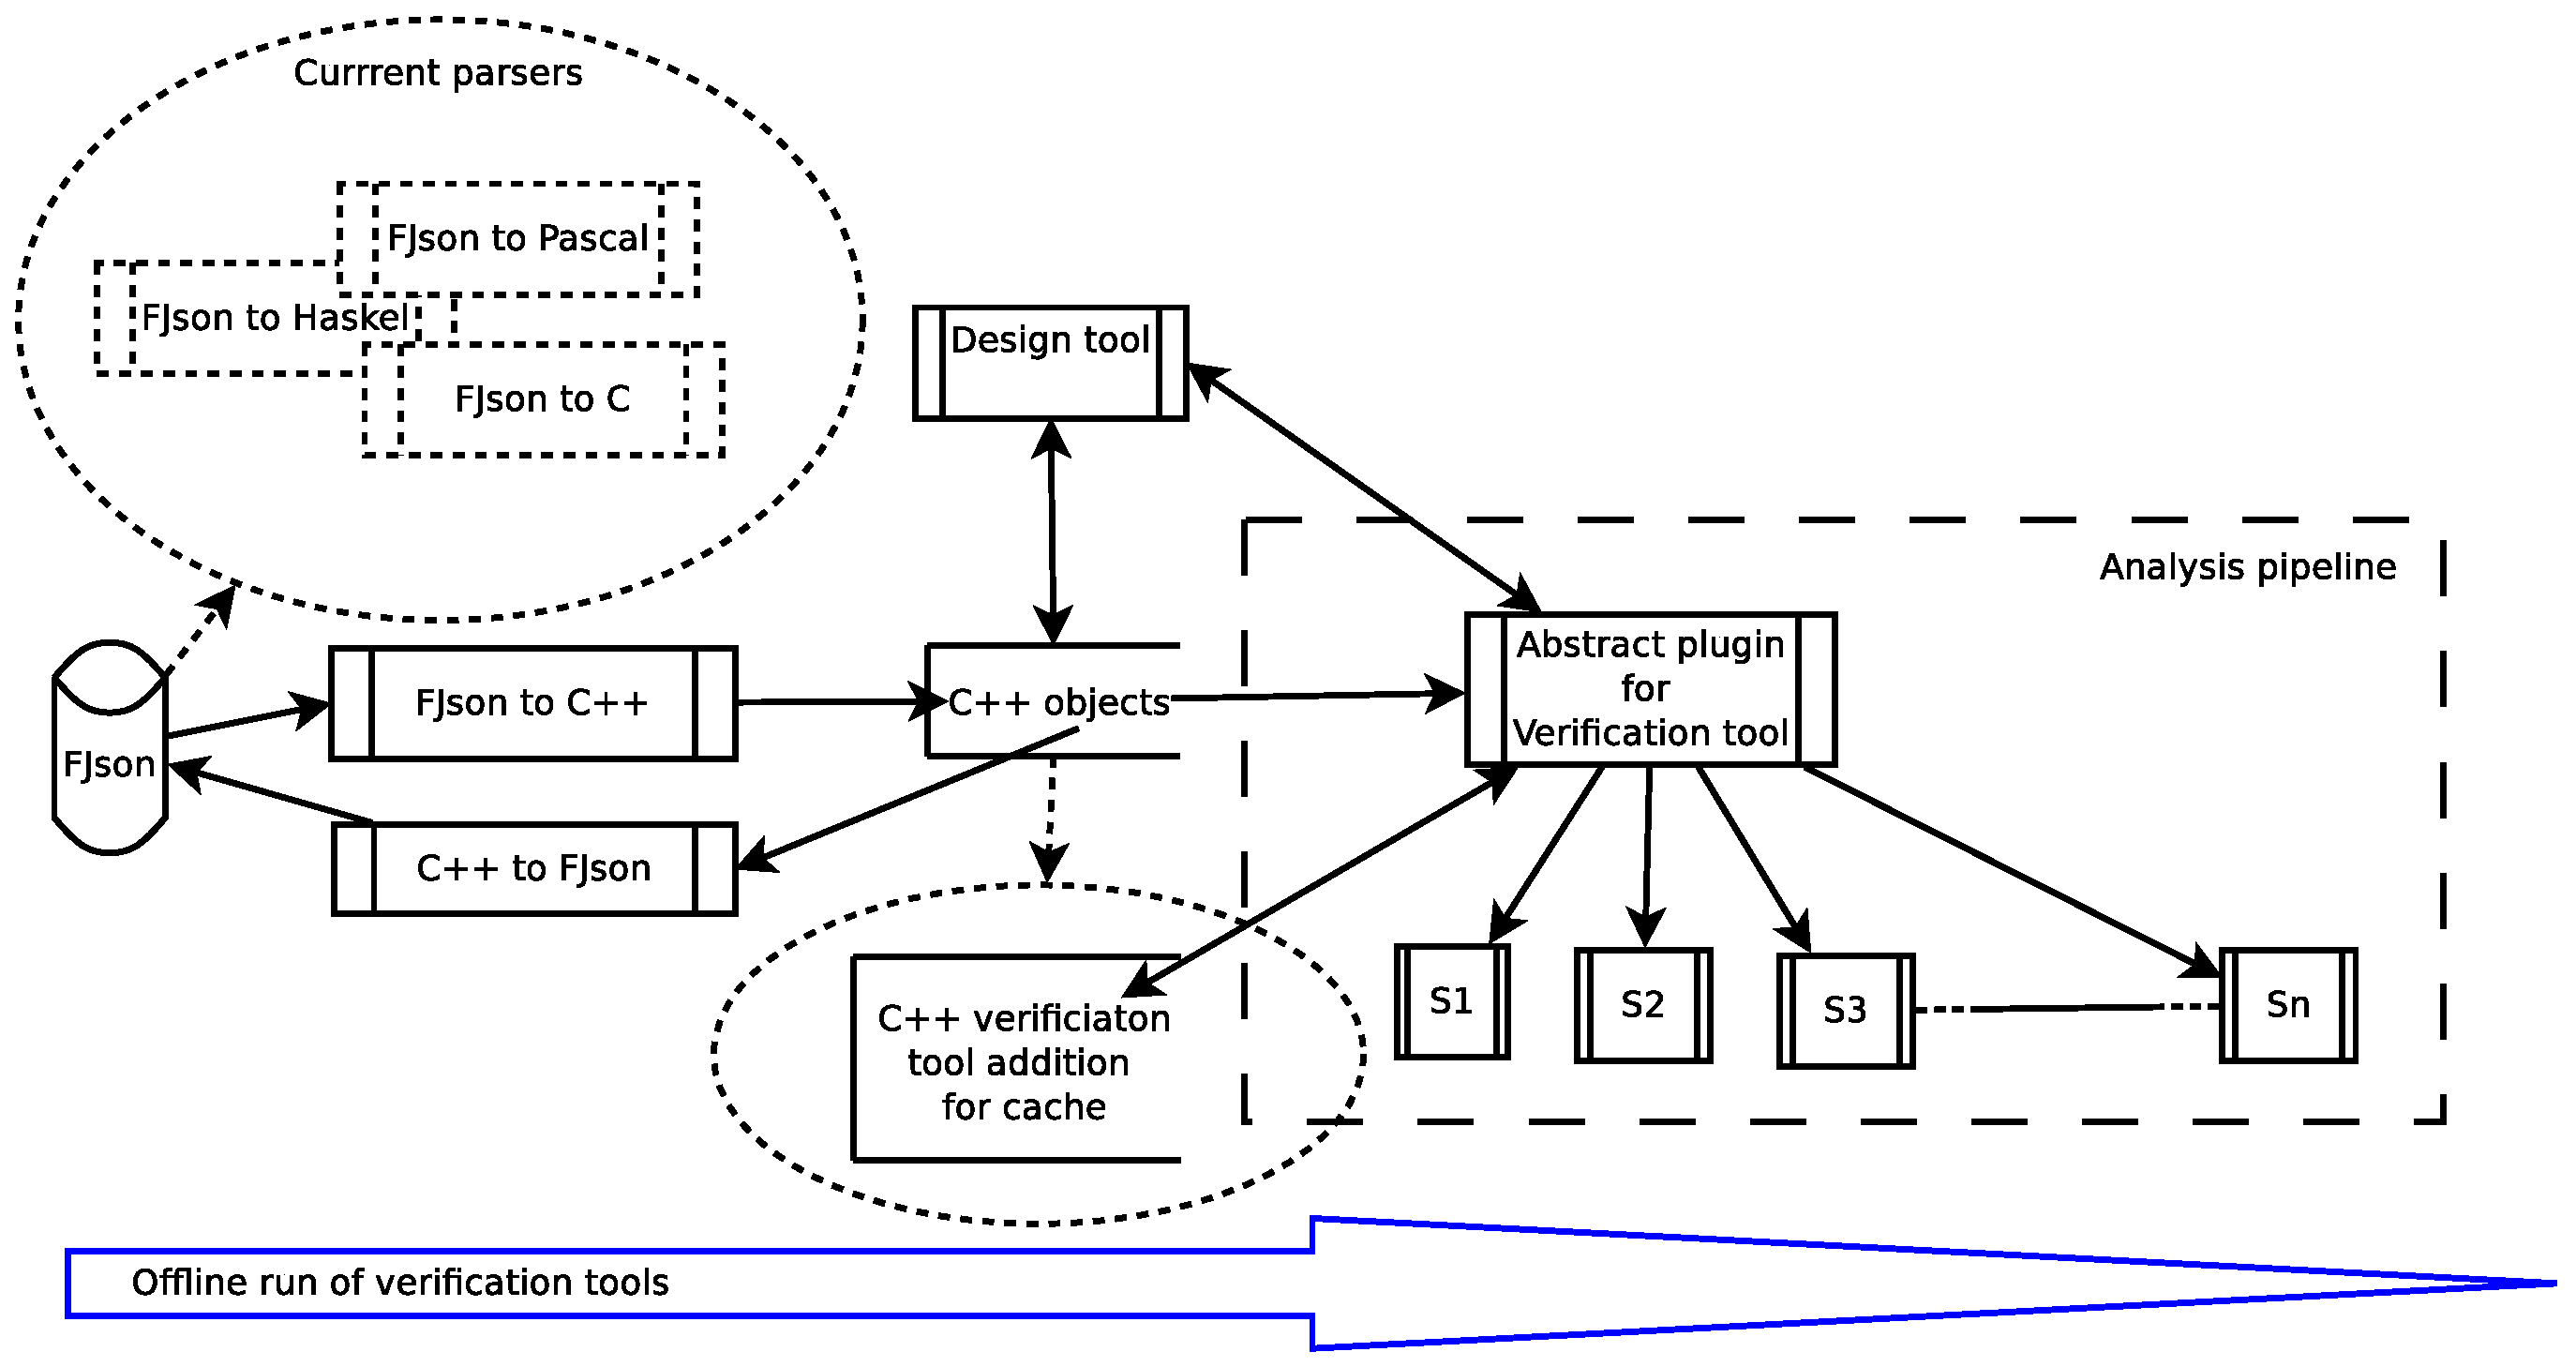
\includegraphics[width=.9\linewidth]{meeting-2014-11-27/2014-11-27-meeting-architecture-tool}
	\captionof{figure}{High level architecture for GUI and pipeline}
	\label{fig:architecture-high-level}
\end{center}

\begin{description} 

	\item[Offline run van verificatie] Vanaf de command line of vanuit een
		script kunnen de onderzoekers alle verificitie tools draaien over een
		model om de uitvoer via logfiles te verzamelen dan wel op standaard
		output te krijgen. Deze batch run is noodzakelijk bij het
		verifi\"{e}ren van grotere modellen. Men voert dit ook wel 's nachts
		uit.

	\item[Online run van verificatie] Bij het gebruik van het online design
		tool moet men selectief verificatie tools kunnen kiezen.  De in te
		vullen parameters hangen direct samen met de geselecteerde tools.
		
	\item[plugin architectuur] De plugin architectuur is iets dat de
		verificatie stappen uitvoert voor 1 of meer verificatie tools. De
		werking en samenhang van de verificatie tools zelf is buiten scope. De
		plugin architectuur en de generieke plugin code is in scope. Het doel
		van de plugin is de hoeveelheid boilerplate code te minimaliseren en
		het gemak van introduceren van een nieuw tool te maximalieren.
		
	\item[Plugin communicatie] De communicatie tussen plugin en ontwerp tool is
		onderwerp van discussie. De ideeen zijn gebruik te maken van pipes of
		van zeroMQ. Het voordeel van zeroMQ is platform onafhankelijkheid
		terwijl zeroMQ ook gebruik maakt van pipes als de processen op dezelfde
		machine draaien.
	
	\item[Current parsers] Op dit moment zijn er meerdere parsers van FJson
		naar interne structuren. Het doel van Bernard is het aantal parsers tot
		\'e\'en te beperken: die van en naar een C++ structuur. Tevens is dit
		de enige datastructuur zodat verschillen in semantiek tot het verleden
		behoren.

	\item[C++ verification tool addition] De huidige C++ datastructuur bevat
		behalve gegevens voor het model ook gegevens voor de verificatie tools.
		Het doel is caching zodat verificatie minder lang duurt.  Het is ter
		discussie of deze gegevens in het C++ model thuishoren dan wel ergens
		anders bij de verificatie modules thuis horen.  

	\item[Additionele libraries] Voor process control en thread control moeten
		we i.v.m. platform onafhankelijkheid leunen op tools die threads en
		processen platform onafhankelijk kunnen aansturen. De ideeen gaan
		uit naar de library \w{Boost}. Zie opmerking in volgend topic over 
		code van Bernard uit \w{Boost}

\end{description}

\topic{Diverse onderwerpen}

\subtopic{Efficientere programmering}

Bernard heeft tijdens zijn promotieproject code ontwikkeld die effici\"{e}nter
omgaat met diverse C++ zaken. Dit betreft onder andere strings (een efficiente
vorm die je goedkoper kunt kopieren vergelijkbaar met bstring), en onderdelen
van de boost library. Op verzoek kan hij ons hier mee helpen.

\subtopic{Domain analysis user interface toolkits}

Bernard heeft de domein analyse volledige gelezen en is het met onze keuze voor
FLTK eens. 

\subtopic{Boost} Over het gebruik van \w{Boost} waarschuwt Bernard dat deze onder
apple alleen in zijn geheel te installeren is. Als ik het goed heb begrepen
moeten alle \w{Boost} libraries vanuit source gecompileerd worden: dat duurt lang.
Voor Linux en Windows is dit probleem er niet. Bernard heeft voor een ander
project code uit \w{Boost} ge\"{i}soleerd, dat wij kunnen gebruiken.

\subtopic{0mq} Over \w{zeroMQ} is Bernard gematigd terughoudend. De library heeft een goede
reputatie, maar de voordelen voor ons project zijn beperkt tot platform onafhankelijkheid.
Omdat platform onafhankelijkheid wel erg belangrijk is en gebruik van \w{0MQ} geen
merkbare nadelen heeft, lijkt dit een goede keuze.

\subtopic{Git repository}

Bernard geeft aan een kopie te gaan maken van onze huidige github repository. We kunnen 
voorlopig gebruik blijven maken van de github repo. De git repo van de OU werkt nog niet.


\end{Minutes}
\end{document}
